\documentclass{article}
\usepackage[utf8]{inputenc}
\usepackage{amsmath, amssymb}
\usepackage[subpreambles=true]{standalone}
\usepackage{graphicx}
\usepackage{geometry}
\usepackage{wrapfig}
\usepackage[most]{tcolorbox}
\usepackage{titlesec}
\usepackage{booktabs}
\usepackage{float}

\geometry{margin=1in}
\newcommand{\sectionbreak}{\clearpage}

\usepackage{hyperref}
\hypersetup{
    colorlinks=true,
    linkcolor=blue,
    filecolor=magenta,      
    urlcolor=blue,}
    
\begin{document}
\newcommand{\calG}{\mathcal{G}}
\title{Physics 742: \\
	Statistical Mechanics \& Condensed Matter\\
	Notes on statistical mechanics and complex networks}

\author{Dion O'Neale, Frazer Moore, Maxwell N. Finan-Jenkin, \\
Alex Ferguson, W. Liao, Jasmine Anderson-Baldwin, Juliet Nelson,\\
Gray Hunter, Fadi Wassaf}

\maketitle
\newpage
\tableofcontents
\newpage

\input{01-thermodynamicsRefresher.tex}
\input{02-probability.tex}
\input{03-statisticalPostulates.tex}
\input{04-hamiltonianPhaseSpace.tex}
\input{05-molecularDynamics.tex}

\input{06-ensembles.tex}
\section{Quantum statistical mechanics}

\newcommand{\bra}[1]{\langle #1 |}
\newcommand{\ket}[1]{| #1 \rangle}
\newcommand{\braket}[2]{\langle #1 | #2\rangle}

In this section we want to extend the classical statistical mechanics concepts that we have seen so far to quantum mechanical systems. When we do so, we will find that two particular properties of quantum systems --- the (anti-)symmetry of the wave function for fermions (resp. bosons), and the indistinguishability of particles --- have consequences for the statistics of the ensembles that they are part of.

First though we will motivate the investigation of quantum systems by looking at the case of ensembles of classical and quantum harmonic oscillators.
\subsection{Classical and quantum harmonic oscillators}
A collection of $N$ classical simple harmonic oscillators is described by the Hamilitonian
\[
	H(p_i,q_i) = \frac12m\omega^2q_i^2+\frac{1}{2m}p_i^2,\quad i=1,2,3,\ldots,N
\]
where $\omega^=\kappa/m$ and $\kappa$ is the spring constant for the oscillators.

For a single oscillator, the partition function is given by 
\[
	Z_1 = \frac{1}{h}\int_{-\infty}^{\infty} \int_{-\infty}^{\infty}\exp\left[-\beta(\frac12m\omega^2q^2+\frac{1}{2m}p^2)\right]\mathrm{d}p\mathrm{d}q.
\]
We can split this in to two Gaussian integrals and get
\[
	Z_1 = \frac{1}{h}\sqrt{2\pi/(\beta m\omega^2}\sqrt{2\pi m/\beta} = \frac{1}{\beta\hbar\omega}.
\]
From this we can write down the expression for the system of N independent and distinguishable oscillators:
\[
	Z = Z_1^N = (\beta\hbar\omega)^{-N}.
\]
The Helmholtz free energy for such a system is given by
\[
	F = -kT\ln(Z_N) = NkT\ln\left(\frac{\hbar\omega}{kT}\right)
\]
and similarly
\[
	E = \frac{-\partial}{\partial\beta}\ln(Z) = NkT.
\]
The energy per oscillator is therefore $E/N = kT =\langle E_1 \rangle$. This is an example of the \emph{equipartition theorem}.

\subsubsection{The equipartition theorem}
Assume that:
\begin{itemize}
	\item The system is classical. That is $kT>$ is much greater than the spacing between quantum levels.
	\item	The system includes at least one variable that has a quadratic contribution to the total energy. That is $H(q_i,p_i) =\alpha x^2 +\widetilde{H}(q_i,p_i)$ where $x$ is one of the variables in the set of $\{q_i,p_i\}$ that is not in the $\widetilde{H}$ term.
\end{itemize}
Then, $\langle\alpha x^2\rangle = \frac12kT$.

Proof: You do it! Start with $\langle\alpha x^2\rangle = \frac{\int \mathrm{d}p\mathrm{d}q \exp(-\beta H)\alpha x^2}{\int \mathrm{d}p\mathrm{d}q \exp(-\beta H)}$.

The consequence of the equipartition theorem is that when a system is in thermal equilibrium, each variable has a quadratic term only in $H$ and contributes $kT/2$ towards the total energy $E$. Therefore, for a system of $N$ harmonic oscillators the total energy is $NkT$, since each oscillator has a quadratic term for both the kinetic and potential terms.

Now, let's consider a quantum harmonic oscillator where $\omega$ can take only discrete values. The energy eigenvalues of the oscillator are $\epsilon_n = (n+\frac12)\hbar\omega$, $n=0,1,2,\ldots$. The Hamiltonian for a single oscillator is therefore given by
\[
	Z_1 = \Sigma_{n=0,1,2,\ldots}\exp(-\beta H) =  \Sigma_{n=0,1,2,\ldots}\exp(-\beta(n+\frac12)\hbar\omega) = \frac{\exp(-\beta\hbar\omega/2))}{1-\exp(-\beta\hbar\omega))}
\] 
where the last equality comes from treating the sum as a geometric series.
From this, we have
\[
	\ln(Z_1) = -\frac12\beta\hbar\omega -\ln(1-exp(-\beta\hbar\omega))
\]
so the partition function for $N$ independent oscillators is
\[
	Z_N(\beta) = Z_1(\beta)^N = exp(-N\beta\hbar\omega/2)\left(1-\exp(-\beta\hbar\omega)\right)^{-N} 
\]
and the Helmholtz free energy is
\[
	F = N\left[\frac12\hbar\omega + kT\ln(1-\exp(-\beta\hbar\omega))\right].
\]
We'd like to see what the consequences of quantization are on the equipartition theorem, so we calculate the total energy
\[
	E = \frac{-\partial}{\partial \beta}\ln(Z) = N\left[\frac12 \hbar\omega + \frac{\hbar\omega}{\exp(\beta\hbar\omega) - 1}\right].
\]

Now, consider the limit $\beta\hbar\omega = \frac{\hbar\omega}{kT} << T$, that is, $kT$ and hence the temperature is large with respect to $\hbar\omega$, the separation of energy levels for the quantum oscillator. In this regime $\exp(\beta\hbar\omega)\simeq 1+\beta\hbar\omega$, the mean energy of the system is
\[
	E \simeq \hbar\omega\left(\frac12 + \frac{1}{\beta\hbar\omega}\right) \simeq \hbar\omega\left(\frac{1}{\beta\hbar\omega}\right) = kT.
\]
That is, we recover the classical result for the equipartition theorem when $kT$ is large.

The `cold' limit has $\beta\hbar\omega = \frac{\hbar\omega}{kT}>>1$ and hence $\exp(\beta\hbar\omega)>>1$. In this case the mean energy of the system is
\[
	E\simeq \hbar\omega\left(\frac12\exp(-\beta\hbar\omega\right) \simeq\frac12\hbar\omega
\]
so the mean energy approaches the ground state, or zero point energy. [A more accurate approximation gives $E\simeq \frac12\hbar\omega+\hbar\omega\exp\left(\frac{-\hbar\omega}{kT}\right)$ which accounts for excitations of the oscillators to the state $\epsilon_1 = \hbar\omega(\frac12+1)$ which occur with probability $p\propto\exp(-\beta\hbar\omega)$.]


\subsection{Quantum statistical mechanics of non-interacting particles}

In quantum mechanics we already have two layers of uncertainty about the state of a system: the Heisenberg uncertain principle $\Delta{p}\Delta {r}>{\hbar}/{2}$ means that rather than having a discrete point in phase space to describe the state of a system, the most precision we can hope for is some small region in phase space, centered on that point. Quantum mechanics also deals with probability distributions itself: the wave function $\psi_n({\bf r})$ (or rather $|\psi_n|^2$) describes the probability distribution of a particle being in a particular quantum state.

Statistical mechanics adds an extra layer of probability to this situation in order to deal with ensembles that have probabilities $p_n$ of being in a variety of quantum states $\psi_n$. These quantum ensembles are called \emph{mixed states}. They are distinct from the superposition of quantum states. The superposition of two wave functions implies that the system is in a state comprised of both wave functions simultaneously, while the mixed state says that the system could be in one state or the other, or perhaps both. For example: if $\ket{H}$
is the wave function for a horizontally polarized photon and $\ket{V}$ is the wave function for a vertically polarised photon, then the superposition $\frac{1}{\sqrt{2}}(\ket{H}+\ket{V})$ is a diagonally polarised photon, while the mixed state is an unpolarised photon that is half $\ket{H}$ and half $\ket{V}$ that could be in either state:  i.e. $\frac12\left(\ket{H}\bra{H}+\ket{V}\bra{V}\right)$.

Given a quantum system in a particular state, represented by the wave function $\psi_n$, the quantum expectation of an operator $\hat{A}$ is given by
$$
	\langle\hat{A}\rangle_\text{QM} = \int\psi^*_n\hat{A}\psi_n.
$$
(I'll try to always use hats to denote quantum operators, but I'll probably forget them from time-to-time.)

This is sometimes also denoted as $\langle\hat{A}\rangle_\text{pure}$ as it applies to a purely quantum state, where no possibilities of different statistical mechanical configurations exist.

The statistical mechanical expectation operator for an ensemble is given by
$$
		\langle\hat{A}\rangle = \sum_n p_n\int\psi_n^*\hat{A}\psi_n.
$$
Quantum statistical mechanics is concerned with figuring out how the properties of $\psi_n$ affect the expected value of $\hat{A}$.

\subsubsection{A refresher: bra-ket notation}
The bra-ket notation, popularised by Dirac, gives us an extremely convenient and compact way of dealing with elements of a vector space (in QM, a Hilbert space) in various combinations. It doesn't introduce any new physics but it does let us, for example, use the same notation for an inner product of two quantities, whether they are finite-dimensional vectors or infinite dimensional functions.

$\ket{v}$ by itself (pronounced ket $v$) is just the column vector (or function) $v$.

$\bra{u}$ by itself (pronounced bra $u$) is interpreted as the conjugate transpose of $\ket{u}$, i.e. $\bra{u}=\ket{u}^*$.

The notation becomes particularly convenient when we want to calculate inner products
$$
	\braket{u}{v} = u^*v
$$
for finite dimension vectors or 
$$
	\braket{u}{v} =	\int d{\bf r}u^*({\bf r})v({\bf r})
$$
for functions.

Similarly, the outer product can be denoted 

$$
\ket{u}\bra{v}=uv^* =
\begin{bmatrix}
    u_1v^*_1 & u_1v^*_2  & \dots \\
    u_2v^*_1 & u_2v^*_2  & \dots   \\
    \vdots & \vdots & \ddots 
\end{bmatrix}.
$$

For an operator $\hat{A}$ acting on a ket $\ket{v}$ we have $\hat{A}\ket{v} = \ket{\hat{A}v}$ and hence 
$$
	\bra{u}\hat{A}\ket{v}=\braket{u}{\hat{A}v} = u^*\hat{A}v
$$
Or, equivalently,  
$$
	\braket{u}{\hat{A}v} = \int d{\bf r} u^*({\bf r}) \hat{A} v({\bf r}).
$$

Bra-ket notation has a number of convenient properties; one that we will make use of shortly is that closed bra-ket sets commute with each other. This is easy to see by considering the vector case where a closed bra-ket pair is just a scalar.

\subsubsection*{The density matrix/density operator}
Similar to the way that the single particle density is a convenient way of introducing a probability density into classical statistical mechanics, the density matrix $\rho = \sum_n p_n\ket{\psi_n}\bra{\psi_n}$ (or the density operator $\hat{rho}$ in the case of functions) allows us to consider a probability distribution over an ensemble of quantum states.

To see how the density matrix arises, we will begin with the expression we had earlier for the ensemble expectation of an observable corresponding to some operator $\hat{A}$, which we can now write in bra-ket notation.
\begin{equation}
	\langle\hat{A}\rangle = \sum_n p_n\bra{\psi_n}\hat{A}\ket{\psi_n}.
	\label{eq:7.2}
\end{equation}
(We are going to assume throughout this section that all the vectors/wave functions that we deal with have already been normalised.) Now, if $\phi_a$ is any orthonormal basis then the identity operator is
$$
	Id = \sum_a\ket{\phi_a}\bra{\phi_a}.
$$
If we insert this into equation (\ref{eq:7.2}) for the expected value of $\hat{A}$ we get
\begin{eqnarray*}
	\langle\hat{A}\rangle &=& \sum_n p_n\bra{\psi_n} \left(\sum_a\ket{\phi_a}\bra{\phi_a}\right) |\hat{A}\ket{\psi_n}\\
	&=& \sum_n p_n\sum_a\bra{\phi_a}\hat{A}\ket{\psi_n}\braket{\psi_n}{\phi_a}\\
	&=& \sum_a \bra{\phi_a}\hat{A} \left(\sum_n p_n \ket{\psi_n}\bra{\psi_n}\right)\ket{\phi_a}\\
	&=& \sum_a \bra{\phi_a}\hat{A}\rho\ket{\phi_a}\\
	&=& \text{Tr}(\hat{A}\rho)
\end{eqnarray*}
where $\text{Tr}(M)$ denotes the trace of $M$ (in the case of a matrix, this is the sum over the diagonal elements).
Normalisation means that we have $\text{Tr}(\rho)=1$ and $\sum_n p_n=1$.

We can now use the density matrix to give some expressions for the quantum [micro-$|$grand-]canonical ensembles.

\subsection{Quantum micro-canonical ensemble}
We will consider a system with fixed $N$ and $V$. Because we are dealing with a quantum system, rather than fixing the total energy of the system we fix the interval $(E,E+\epsilon)$ where $\epsilon$ is some (small) uncertainty. We will denote by $E_j$ the (discrete) energy eigenstates that correspond to the Hamiltonian operator $\hat{H}$.

The system has distinct accessible micro-states that correspond to the macro-state $(N,V,E;\epsilon)$. The number of distinct accessible states is given by counting over the phase space to get $\Gamma(N,V,E;\epsilon)$. We are going to assume that the probability of the system being in any of the energy states in the interval is equal --- this is the so-called \emph{equal a priori postulate}.

The probability of the system being in a particular micro-state $E_j$ is therefore
$$
	p(E_j) =
	\begin{cases}
		\frac{1}{\Gamma} \text{ if } E<E_j<E+\epsilon\\
		0 \text{ otherwise}
	\end{cases}
$$
and, if we choose a basis such that the Hamiltonian operator $\hat{H}$ is diagonal, then the density matrix is the diagonal matrix
$$
	\rho = \sum_j p(E_j) \ket{E_j}\bra{E_j}.
$$

The entropy is given by
$$
	S(E) = k_B\ln\Gamma(E).
$$
At this point, it's worth noting that when we count the states that comprise $\Gamma$ we must do so in a quantum fashion, i.e. taking account of the indistinguishability of the quantum particles.

We can also write this in a form similar to that for the Gibbs entropy that we saw in an earlier section:
$$
	S(E) = -k_b\sum_jp(E_j)\ln(p(E_j))=-k_B\text{Tr}(\rho\ln\rho).
$$ 

\subsection{Quantum canonical ensemble}
Here we take:
$$
	p(E_j) = \frac{1}{Z}\exp\left(\frac{-1}{k_BT}E_j\right)
$$
and
$$
	Z = \sum_j \exp\left(\frac{-1}{k_BT}E_j\right).
$$

Again, if we assume, that we have picked a basis where $\hat{A}$ is diagonal and has energy eigenstates $E_j$ (i.e. $\hat{H}\ket{E_j} = E_j\ket{E_j}$) then, we can write
$$
	\rho = \frac{1}{Z}\exp\left(\frac{-1}{k_BT}\hat{H}\right)
$$
where
$$
	Z = \text{Tr}\left[\exp\left(\frac{-1}{k_BT}\hat{H}\right)\right].
$$

\subsection{Quantum grand-canonical ensemble}
The density matrix is given by
$$
	\rho = \frac{1}{Z}\exp\left(\frac{-1}{k_BT}(\mu\hat{N}-\hat{H})\right)
$$
with the corresponding partition function
$$
	Z = \text{Tr}\left[\exp\left(\frac{-1}{k_BT}(\mu\hat{N}-\hat{H})\right)\right].
$$

\subsection{Systems of indistinguishable particles}
This is where we will see one of the more interesting consequences of quantum mechanics on statistical mechanics - namely how the symmetry of the wave function for the particles in our system affect the statistics of the system.

We will consider a system of $N$ identical non-interacting particles --- an ideal quantum gas. Since the particles are non-interacting, the overall Hamiltonian $\hat{H}$ for the system is just the sum of the Hamiltonians for each of the individual particles:
$$
	\hat{H}({\bf q},{\bf p}) = \sum_i^N\hat{H_i},
$$
where $\hat{H}_i$ is the Hamiltonian of the $i$-th particle.

The time-independent Schr\"odinger equation for the system is
$$
	\hat{H}\ket{\psi_E} = E\ket{\psi_E}
$$
where $E$ is an energy eigenvalue of $\hat{H}$ and $\psi_E$ is the corresponding eigenfunction.

We can use the fact that $\hat{H}$ is a sum of non-interacting terms to write the solution $\psi_E$ as a product of the solutions to each of the individual particles: 
$$
	\psi_E = \prod_{i=1}^Nu_{\epsilon_i}
$$
where $\sum_{i=1}^N\epsilon_i = E$ and where $u_{\epsilon_i}$ is the eigenfunction of $\hat{H_i}$, i.e. $\hat{H_i}u_{\epsilon_i}={\epsilon_i}u_{\epsilon_i}$.

Since the stationary state of the overall system can be described in terms of the constituent particles, we just need to specify how many particles are in each energy state. We write $n_i$ for the number of particles in the state with energy $\epsilon_i$ and $\{n_i\}$ for the set of all such $n_i$. We therefore have
$$
	\sum_i n_i =N \qquad \text{and} \qquad \sum_in_i\epsilon_i = E.
$$

The wave function for the overall state can now be written in terms of the particles in each of the distinct energy eigenstates
\begin{equation}
	\psi_E = \prod_{m=1}^{n_1}u_1(m)\prod_{m=n_1+1}^{n_1+n_2}u_2(m)\cdots
	\label{eq:compfn}
\end{equation}
where $u_i(m)$ is the single particle wave function $u_{\epsilon_1}({\bf q}_m)$.
That is, $\psi_E$ is the product of individual particle eigenfunction, each with degeneracy that corresponds to the number of particles in each energy state.
We will refer to this as the Boltzmann wave function, which we will denote $\psi_\text{Boltz}$.

Since the particles are identical, it is possible to permute their coordinates in (\ref{eq:compfn}) while keeping the system in the same state. I.e. the sequence of indices $(1,2,3,\ldots,N)$ are permuted to $(P1,P2,P3,\ldots,PN)$ where $P$ denotes mapping an index $m$ to the permuted index $Pm$. The resulting wave function will then be
\begin{equation}
	P\psi_E = \prod_{m=1}^{n_1}u_1(Pm)\prod_{m=n_1+1}^{n_1+n_2}u_2(Pm)\cdots.
	\label{eq:permfn}
\end{equation}


In classical statistical mechanics, though the particles may be identical, we treat them as being distinguishable. That is, permutation of two identical particles corresponds to two different, though identical, micro-states of the system with the same energy. (This is what leads to the necessity of introducing the Gibbs factor in classical statistical mechanics when evaluating the free energy of the canonical ensemble.  The Gibbs factor $\frac{1}{n_1!n_2!\cdots}$ allows us to correct for the fact that the particles being permuted are \emph{effectively} indistinguishable and the permutation doesn't really correspond to a different micro-state of the system.

In quantum mechanics, the particles are, \emph{in reality} indistinguishable. I.e. all that matters is the number of particles in each state --- the micro-states that occur from permutation are the same micro-state.
Interchanging particle coordinates (i.e. the arguments of $u_i$) in the wave function (\ref{eq:compfn}) should, therefore, not lead to a new micro-state.

How can we make sure that the wave function $\psi_E$ doesn't change under any of the above permutations? One way is to make $\psi_E$ be a linear combination of all the $N!$ possible wave functions that can be formed from such permutations such that the probability density for the quantum system stays the same: $|P\psi|^2=|\psi|^2$.

There are two ways to satisfy this condition. The first is when $\psi$ is symmetric in all its arguments such that $P\psi = \psi$ for all possible permutations. The second way is when $\psi$ is anti-symmetric in its arguments such that
$$
	\psi = 
	\begin{cases}
		+\psi \text{ if $P$ is an even permutation, or}\\
		-\psi \text{ if $P$ is an odd permutation.}
	\end{cases}
$$

We will denote these solutions as $\psi_S$ and $\psi_A$ respectively. They can be written in terms of the Boltzmann wave function (\ref{eq:compfn}) as
$$
	\psi_S=c\sum_P P\psi_\text{Boltz}
$$
and
$$
	\psi_A=c\sum_P \delta_PP\psi_\text{Boltz}
$$
where $c$ is a normalisation constant and $\delta_PP$ is $+1$ or $-1$ depending on whether $P$ is an even or odd permutation, respectively.

The wave function $\psi_A$ can be written as the \emph{Slater determinant} 
$$
	\Psi_A = c\det\begin{bmatrix}
		u_i(1) & u_i(2) & u_i(3) & \dots & u_i(N)\\
		u_j(1) & u_j(2) & u_j(3) & \dots & u_j(N)\\
		u_k(1) & u_k(2) & u_k(3) & \dots & u_k(N)\\
		\vdots & \vdots & \vdots & \ddots & \vdots \\
		u_z(1) & u_z(2) & u_z(3) & \dots & u_z(N)
	\end{bmatrix}
$$

When calculating the terms in the expansion of the determinant, the leading diagonal is the Boltzmann wave function (\ref{eq:compfn}) while the other terms are permutations of it. The signs for the permuted terms appear automatically in the right order as the determinant is calculated.

Exchanging a pair of arguments in the wave function is the same as swapping a pair of columns of the matrix and causes the sign of the contribution to the determinate to change.

If two or more particles are put into the same energy state, then the matrix has two or more identical rows and the determinant becomes zero --- the wave function vanishes. This implies that an anti-symmetric wave function corresponds to a quantum system where no two particles can be in the same state, i.e. the Pauli exclusion principle that applies to fermions. The statistics governing such systems are called \emph{Fermi-Dirac statistics}.

For Fermi-Dirac statistics the weight factor $W_{F.D.}\{n_i\}$ for the state of the system is given by
$$
	W_{F.D.}\{n_i\} = 
	\begin{cases}
		1 \text{ if } \sum_i n_i^2 = N\\
		0 \text{ if } \sum_i n_i^2 > N
	\end{cases}
$$


For symmetric wave functions, there is no such restriction on the number of particles per state $n_i$ and the resulting statistics are called \emph{Bose-Einstein statistics}.

Here the weight factor is
$$
	W_{B.E.}\{n_i\} = 1,\qquad i=0,1,2,\ldots.
$$

It is worth noting that although the properties we derived here all assumed systems of non-interacting particles, the same basic properties hold for systems of interacting particles where, even though the wave function for the system $\psi({\bf r})$ can not be expressed in terms of single-particles wave functions $u_i(r_m)$, it will nevertheless be either symmetric or anti-symmetric, resulting in either Bose or Fermi statistics.



\subsection{Fermionic and bosonic partition functions}
With what we have now covered on non-interacting quantum particles, in combination with what we learnt in the previous section on classical ensembles we are now in a position to introduce the quantum version of the partition function. We wil jump straight to the most commonly used case --- the fermionic and bosonic grand canonical partition functions.

\subsubsection{Bose-Einstein Statistics}
For bosons, all fillings $n_k$ of the energy levels are allowed. Each particle in eigenstate $\psi_k$ contributes energy $\epsilon_k$ and chemical potential $\mu$, so for each particle the partition function is
$$
	Z_k^\text{boson} = \sum_{n_k=0}^\infty\exp(-\beta(\epsilon_k-\mu)n_k) = \sum_{n_k=0}^\infty\left(\exp(-\beta(\epsilon_k-\mu))\right)^{n_k} = \frac{1}{1-\exp(-\beta(\epsilon_k-\mu))}.
$$

The partition function for the ensemble is therefore
$$
	Z^\text{boson} = \prod_{k=0} \frac{1}{1-\exp(-\beta(\epsilon_k-\mu))}.
$$

The expected number of particles in each state can be calculated as
$$
	\langle n_k \rangle^\text{boson} = -\frac{\partial}{\partial \mu}(-\beta\ln(Z)) = \frac{1}{\exp(\beta(\epsilon_k-\mu))-1}.
$$

\subsubsection{Fermi-Dirac statistics}
For fermions where $n_k=0$ or $n_k=1$ the single particle partition function is
$$
	Z_k^\text{fermion} = \sum_{n_k=0}^1 \exp(-\beta(\epsilon_k-\mu)n_k) = 1 + \exp(-\beta(\epsilon_k-\mu)),
$$
and the partition particle for an ensemble is
$$
	Z^\text{fermion} = \prod_k(1+ \exp(-\beta(\epsilon_k-\mu))).
$$
The expected number of fermions per state is therefore
$$
		\langle n_k \rangle^\text{fermion} = \frac{1}{\exp(\beta(\epsilon_k-\mu))+1}
$$

\subsubsection{Maxwell-Boltzman statistics}
Maxwell-Boltzman statistics describe the distribution of classical particles, however they are sometimes still useful in the context of quantum systems. (Partly because the maths for them is typically slightly simpler). The Maxwell-Boltzman statistics arise from initially treating particles as being distinguishable, but then dividing the number of micro-states by $N\!$ to account for the double-counting of states that results from doing this. This transformation to the statistics of indistinguishable particles amounts to the so-called dilute limit of M-B statistics in which F-D and B-E statistics are equivalent. The way to think about this is that if you have a large number of states for a small number of particles, even in a classical distribution there is a vanishingly small probability of having more than one particle per state, thus the F-D and B-E statistics are equivalent in this limit.

The partition function for M-B statistics is the familiar
$$
	Z^{MB}_{ensemb} = \prod_k \exp(-\beta(\epsilon_k-\mu))
$$
and the expected number of particles in the $k$th energy state is
$$
\langle n\rangle_{MB} = \exp(-\beta(\epsilon_k-\mu)).
$$

%\subsection{An example: the quantum harmonic oscillator}
%We are going to consider a quantum harmonic oscillator (QHO) with frequency $\omega$ and energy levels $E_n = (n\frac12)\hbar\omega$.

%The partition function for the QHO is $Z^\text{QHO} = \sum_n\exp(-\beta E_n)$, where for convenience, I've put $\frac{1}{k_BT} = \beta$. Writing this out in full and exploiting the fact that we have a geometric series $\sum_n x^n = \frac{1}{1-x}$ we get
%\begin{eqnarray*}
%	Z^\text{QHO} &=& \sum_{n=0}^\infty \exp(-\beta\hbar\omega(n+\frac12))\\
%	&=& \exp(-\beta\hbar\omega/2)\sum_{n=0}^\infty(\exp(-\beta\hbar\omega))^n \\
%	&=& \exp(-\beta\hbar\omega/2)\frac{1}{1-\exp(-\beta\hbar\omega)}.
%\end{eqnarray*}

%To find the average internal energy, think back to when we first introduced the partition function to normalize the probability of a particle being in a state with a particular energy $E_n$.

%We have
%$$
%	\langle E\rangle = \sum_n E_n P_n = \frac{\sum_n E_n \exp(-\beta E_n)}{Z} = \frac{-\partial Z}{\partial \beta}\frac{1}{Z} = -\frac{\partial}{\partial \beta}\ln{Z},
%$$

%So,
%\begin{eqnarray*}
%	\langle E\rangle^\text{QHO} &=& -\frac{\partial}{\partial}\ln(Z^\text{QHO})\\
%	&=&  -\frac{\partial}{\partial\beta} \left[\ln\left( \exp(-\beta\hbar\omega/2)\frac{1}{1-\exp(-\beta\hbar\omega)}\right) \right] \\
%	&=& \frac{\partial}{\partial \beta} \left[ \beta\hbar\omega/2 - \ln\left(\frac{1}{1-\exp(-\beta\hbar\omega)}\right)\right]\\
%	&=& \frac{\partial}{\partial \beta} \left[ \beta\hbar\omega/2 + \ln\left({1-\exp(-\beta\hbar\omega)}\right)\right]\\
%	&=& \hbar\omega/2 + \frac{\hbar\omega\exp(-\beta\hbar\omega)}{1-\exp(-\beta\hbar\omega)}\\
%	&=& \hbar\omega\left(\frac12 +\frac{1}{\exp(\beta\hbar\omega)-1}\right)
%\end{eqnarray*}

%and expected value for the excitation level is $\langle n\rangle^\text{QHO} = 1/(\exp(\beta\hbar\omega)-1)$.

\subsection{Recommended reading}
Although I've made lots of use of \emph{Statistical Mechanics in a Nutshell} in other sections of the course, I feel like it does particularly poorly with quantum systems. \emph{Statistical Mechanics made Simple} does better, but it doesn't give much of an overview of the fundamentals. So, for this section I've made use of \emph{Statistical Mechnaics} by R.K. Pathria, particularly the fundamentals in chapter five. Chapters six through eight give more details on ideal quantum systems and Fermi and Bose systems --- have a look at them too. The other useful text is \emph{Entropy, Order Parameters and Complexity} by J.P. Sethna, specifically chapter seven. You should read sections 7.6 and 7.7 for some simple examples on bosonic and fermionic systems. Finally, chapters five and six of SMmS covers bosonic and fermionic systems well once you've got the fundamentals sorted.

\section{Complex networks}

Graph theory is a well established area of mathematics. More recently, other areas from physics to economics, sociology to ecology have found that the structures and properties of graphs give a powerful and practical method of representing systems of interest to them. This new focus on what might have been called applied graph theory is what is now mostly know as network science. One of the interesting aspects of network science is that it deals with structures that are non-regular (not lattice-like) but also not purely random. These heterogeneous patterns of connections have implications for the study of complex systems (systems of entities with non-trivial sets of typically non-linear interactions) and hence networks often get referred to as complex networks. The Complex part of the name is really a bit redundant, but it sounds good and is commonly used, so we'll stick with it.

\subsection{An introduction to graph theory \& networks}

A network or \emph{graph} is a collection of \emph{vertices} (nodes) $V=\{v_i\}$ and \emph{edges} (links) $E=\{e_{ij}\}$ which we denote $G= G(V,E)$.

If we consider the edge $e_{ij}$, between vertices $v_i$ and $v_j$ to be distinct from $e_{ji}$ then we say that the edge is \emph{directed}. A graph is directed if all its edges are directed. A \emph{simple graph} is a network (possibly directed) where there is a unique (directed) edge between connected pairs of nodes. A \emph{multigraph} allows for the possibility of multiple edges edges between the same nodes. We will mostly only consider simple graphs, though much of what we'll present also holds for multigraphs, with a slight adjustment. 

The \emph{density} of a graph is the number of edges present in the graph divided by the number of possible edges. For an undirected simple graph with $|V|=n$ nodes, the density is given by
$$
	\rho = \frac{|E|}{\frac12 n(n-1)},
$$
where $|E|$ is the number of edges and where the factor of $\frac12$ comes from the fact that the edges are undirected so $e_{ij}=e_{ji}$. 

The \emph{degree} of a node in a network, often denoted $k$ or $k_i$ for the degree of node $i$ is the number of edges that connect to that node. In the case of a directed network we have both \emph{in-degree} and \emph{out-degree}, the number of incoming and outgoing links, respectively.

The \emph{component} of a graph to which a vertex belongs is the set of vertices that can be reached from it by paths running along the edges of the graph. A node in a directed graph has both an \emph{in-component} and an \emph{out-component} corresponding to the nodes that it can be reached from and the nodes that can be reached from it. A graph need not consist of only a single component, though some properties are ambiguously defined when it does not.

The \emph{geodesic path} between a pair of nodes is the shortest path through the network that connects them. The shortest path need not be unique and for a directed network the shortest path can differ depending on direction.
It is sometimes interesting to look at the \emph{average shortest path} for a graph. That is the average over all possible shortest paths in the graph, computed for each pair of nodes. 

The notation $e_{ij}$ for the edges of a network suggests that we can represent a network as a matrix. If we let the rows and columns of the matrix represent the vertices of the network, then the non-zero entries of the matrix represent edges between pairs of vertices. We call such a network the \emph{adjacency matrix} of the graph. The values of the non-zero entries can be used to denote \emph{edge weights} of a \emph{weighted graph}.

Many real-world networks consist of nodes of different types, with connection only between nodes of certain types. The simplest example of this is a \emph{bipartite network} (also known as a \emph{two-mode network}): a network of two types of vertices $V=\{v_i\}$ and $U=\{u_j\}$ where the edges only connect nodes of type $v$ to nodes of type $u$. For example, a publication network where $V$ represents authors and $U$ their publications.  (More generally, the two node types are often referred to as agents and artifacts.) Edges link authors to their publications but not publications to publications, nor authors to authors. In order to obtain a co-authorship network from this publication network it would be necessary to calculate the \emph{unipartite} or \emph{one-mode projection} of the bipartite network.


\subsection{Real-world networks: some examples}

{\bf Social networks:} 

A social network is a set of people or groups with some pattern of contacts or interactions between them. They include such diverse examples as friendship networks of dolphins and interactions between characters in works of fiction, through to more traditional networks such as friendships between individuals, either in real life, or on Facebook, employment networks, and business relationships between companies.

Some of these networks, like the business relationships are best viewed as undirected networks, while others, like real-life friendship networks are directed. Friendship networks lend their name to an interesting feature of networks: the so called \emph{friendship paradox} which states that your friends will typically have more friends than you do. This arises from the fact that like many other real-world networks, friendship networks have a heavy-tailed degree distribution so picking a random node and following an edge from it is likely to lead you to a node with higher degree than the starting node.

\emph{Contact networks} are one important example of social networks. These are networks of when people are in close enough proximity to allow for a disease to spread between them. (Close enough obviously depends on the type of disease.) Contact networks play an important role in modeling of disease contagion --- for example the recent Ebola outbreak in West Africa was successfully modeled using contact networks and this played an important role in managing the epidemic. See also: COVID-19



{\bf Information networks:}

These could equally be called knowledge networks. Examples include the publication networks mentioned earlier (bipartite, undirected), citation networks (directed) whether as citations of publications or of patents, and the World Wide Web (directed). (Note --- the WWW should not be confused with the internet; one is a collection of electronic documents that can link to one another, the other is a collection of computers and switches connected by cables.) Preference networks are another example of information networks that are often used in real-world applications. Examples include networks of people linked to their Netflix viewings, or their Amazon purchases. Identifying patterns in such networks and predicting likely new links is a highly active area of both academic and commercial interest.


{\bf Technological \& infrastructure networks:} 

These are networks with physical links between nodes. Examples include the internet (undirected); electricity grids (partly directed) perhaps also including the computers that control the grid; road, rail, shipping, or air transport networks; and electronic circuits. 


{\bf Biological networks:} 

These networks span multiple scales, from networks of interactions between proteins and their metabolites, or genes and proteins (both directed) that are used amongst other things, in the study of disease through to networks of interactions between species. The latter includes food webs (directed) and mutualistic networks like pollination networks (bipartite, directed). Neural networks are another example that is an active area of study; the complete neural network (282 neurons) is known for the nematode C. Elegans. Studying bigger brains, however, requires bigger brains. Though not entirely biological, I'll include in this class a couple of examples of physical networks. These are networks linking free energy minima of glasses via the saddle points on the energy surface that they sit on and networks linking confirmations of polymers when they can transition between a pair of structures. 


\subsection{Properties of networks}

{\bf Small world effect:}

One of the best know network properties is the \emph{small world effect}. This gets it name from a famous experiment in the 1960s by the sociologist Stanley Milgram. In the experiment, letters were passed from person to person until they reached a designated target person. Milgram found that it took on average only about six hops for the letters to reach their destination leading to the so called \emph{six degrees of separation} phenomenon. This small world effect is an example of how particular network structures can provide short paths through the network connecting most pairs of nodes. 

The mean geodesic path length for an undirected network is given by
$$
	L =\frac{1}{\frac12 n(n-1)}\sum_{i\geq j} d_{ij}
$$
where $d_{ij}$ is the geodesic distance between $v_i$ and $v_j$. In the case of disconnected networks, one must make a choice about how to count the contribution of pairs of nodes that are not connected. The Facebook friendship network is one of the best examples of a small world network. Despite having around 1 billion nodes and 100 billion links (i.e. a mean degree of 100) the mean geodesic distance for the Facebook network is only around four.

{\bf Transitivity/clustering:}

In mathematics, a set with a relationship $\sim$ is transitive if $a \sim b,~b\sim c \implies a \sim c$. In the context of networks the relationship means "is connected to". If a network is entirely transitive, then it would consist of totally connected components. More interesting is to measure how close a network is to being transitive by looking at how much clustering it has.

The \emph{global clustering coefficient} for a network is defined as
$$
	C=\frac{3\times\text{\# of triangles}}{\text{\# number of connected triples}}
$$
where a connected triple is a vertex with connections to two other vertices.

It is sometime interesting to look at how the clustery-ness of a network varies over the network, perhaps to study how clustering depends on some node property. To look at this, we use the \emph{local clustering coefficient} for a vertex $v_i$:
$$
	C_i = \frac{\text{\# triangle connected to }v_i}{\text{\# triples centered on }v_i}.
$$
Clearly, $C = \frac{1}{N}\sum_{i=1}^NC_i$.

Now that we've defined the clustering coefficient, we can look a little closer at the small world property.
If we start with a completely regular network (figure \ref{fig1}a) where each node has the same degree $k$ and is connected to its $k$ nearest neighbours we will have a high clustering coefficient, but a relatively long mena geodesic path. If we start to introduce random re-wirings of the network, with probability $p$, by either switching an end of an existing edge (figure \ref{fig1}b) or by introducing new random links (figure \ref{fig1}c), then we find that the mean geodesic path length drops quickly, while the mean clustering coefficient remains close to its original value as the re-wiring probability $p$ increases --- see figure \ref{fig2}. This means that while the long-range connections rapidly reduce the \emph{global} mean path geodesic length, any change to the \emph{local} structure is barely perceptible.

\begin{figure}
	\begin{center}
		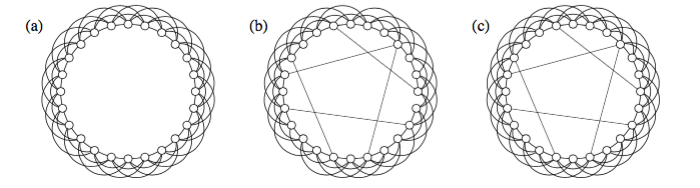
\includegraphics[width = 12cm]{regularNW.png}
	\end{center}
	\caption{}
	\label{fig1}
\end{figure}

\begin{figure}
	\begin{center}
		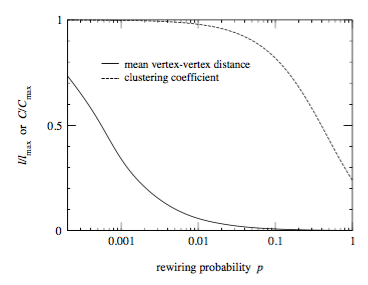
\includegraphics[width = 8cm]{smallWorld.png}
	\end{center}
	\caption{Mean geodesic path length (solid line) and mean clustering coefficient (dashed line) as a function of the rewiring probability $p$, and measured relative to their maximum value, i.e. with no re-wiring.}
	\label{fig2}
\end{figure}


{\bf Degree distribution:}

The degree $k$ of a vertex is the number of edges that connect to that vertex. We write $p_k$ for the fraction of nodes in a network that have degree $k$, this is also the probability that a randomly selected node has degree $k$. One of the interesting properties of real-world networks is the degree distribution --- the histogram of $p_k$ as a function of $k$. For a network with uniformly random connections between nodes, the degree distribution is Poisson. This is not the case for most real-world networks --- these tend to have degree distributions that are highly right-skewed. In particular, many real-world networks tend to have a \emph{heavy-tail} --- a probability distribution that has a non-negligible probability of getting values much greater than the mean. In fact, the mean (and higher order moments like the variance) may not even be well defined for all heavy-tailed distributions.  Of particular interest is the case where the degree distribution is a \emph{power-law} or \emph{scale-free}. That is
$$
 p_k \sim k^{-\gamma}.
$$

Such degree distributions show up surprisingly often in real world networks: the WWW, the internet, metabolic networks, telephone call networks, and sexual contact networks. Power law degree distributions also arise from one of the most popular models for generating networks --- we'll see more on this later.

An alternative (i.e. non-power-law) distribution that is still heavy-tailed is the \emph{exponential distribution}
$$
	p_k\sim\exp(-k/\kappa).
$$

Power-law and exponential distributions are easily identified in data: they give a straight line on log-log and semi-log axes, respectively.

\subsection{Network growth models}
It is one thing to be able to produce a network, fully formed, with a particular set of properties. It is quite another to prescribe a process that is able to grow, or generate, a network with those same properties.

One popular generative network model is the \emph{preferential attachment plus growth model} (PAGP model), also known as the Barabasi and Albert or BA model.

As the name suggests, at each time step, the PAPG model adds a node with degree $m$. Each of the edges of the new node attaches itself to a node in the existing network with a probability that is proportionate to the degree of the existing nodes. The edges in this model are undirected and once and edge is attached to a node, there is no re-wiring. It isn't too hard to prove that the PAPG model generates graphs with a power law degree distribution with $p_k \sim k^{-3}$. The fact that the power law exponent is fixed is unfortunate, though generalisation of the PAPG model allow for different exponents. It is also not hard to see that the PAPG model only produces connected graphs. This limits its applicability to some real world networks. Even though the PAPG model manages to grow networks that reproduce some real-world features (the power-law degree distribution), it does so in a way that may not match up with the growth processes of those real-world networks. For example the highest degree nodes of the PAPG model are the oldest nodes --- this is not the case with networks such as the WWW to which the PAPG model might be applied.

\subsubsection{Recommended reading on growth models}
See the lecture notes by Aaron Clauset on network growth models PDF in the files section of Canvas (not in the reading list).

\subsection{Probability Generating Functions \& Networks}
The probability generating functions that we introduced at the start of the course give a useful way of calculating network properties from their degree distributions. For example, if $G_0(x) = \sum_{k=0}^\infty p_kx^k$ is the PGF for the degree distribution of a network, then the first moment of the PGF gives the average degree, $\langle k \rangle$, of the network, according to
$$
	G_{0}'(x) = \sum_{k}kp_{k}x^{k-1},
$$
and
$$
	G_{0}'(1) = \sum_{k}kp_{k} = \langle k \rangle.
$$	

Another important property is the degree distribution of first neighbours. The reasoning is as follows: by selecting a link at random, and following it until reaching a node, we will find that the node has, let's say, degree $k$. The probability with which we will reach such a node is proportional to its degree ($\propto kp_{k}$). The normalized distribution is given by
$$
	\dfrac{\sum kp_{k}x^{k}}{\sum_{k}kp_{k}} = x \dfrac{\sum kp_{k}x^{k-1}}{\langle k \rangle} = \dfrac{x}{\langle k \rangle}G_{0}'(x).
$$

Then, by following each one of the $k$ edges of a randomly chosen node of degree $k$, we have the distribution of the remaining outgoing edges of the $k$ first neighbours of that node generated by the function 
$$
	G_{1}(x) = \dfrac{\sum_{k}kp_{k}(k)x^{k-1}}{\langle k \rangle} = \dfrac{1}{\langle k \rangle}G_{0}'(x)
$$
Note that because we are following the edges of a randomly chosen node, the distribution of the remaining edges of the first neighbours do not count the edge by which we arrived at that neighbour, hence we get rid of one power of $x$ in the equation for $G_{1}(x)$.

From that, it is not hard to find a new PGF for the number of second neighbours of nodes in a network. 
$$
	\sum_k p_k (G_1(x))^k
$$ 
where 
$$
	G_1(x) = \frac{G_{0}'(x)}{G_{0}'(1)}
$$ 
This, in turn, is close to the PGF for the degree distribution of the projection of a bipartite network, since the second neighbours of a bipartite network are the neighbours of its projection.

\subsection{Exponential random graph models}
Given a particular empirical network one often wants to create models of networks with similar observable properties. These observables might be any of the properties mention so far (or many others) such as mean clustering or a particular degree distribution. One approach is to consider the empirical network as one example of a network from an ensemble of networks that have been generated by the same underlying model. Exponential random graph models (ERGMs) provide a way to study the properties of such models by employing methods that come directly from the statistical mechanics that we have seen so far.

Consider a set $\mathcal{G}$ of graphs and a collection of observables $\{X_i\},~~i=1,2,\ldots,r$ for which we have measured expected values $\langle X_i\rangle$. It will often turn out that we only have a single measurement of these values. (Here we'll assume that the graphs in $\mathcal{G}$ are simple graphs, but the same approach works for many other possibilities.) Given a specific graph $G\in\mathcal{G}$ we want $P(G)$ the probability of finding that graph to be commensurate with the expected values of each of the graph observables $\{X_i\}$. Just like for statistical  mechanics, this is an under-determined problem: the number of degrees of freedom for the definition of $P(G)$ is much smaller than the number of constraints from the observables. However, as we know from statistical mechanics, the best approach is to pick the solution that maximises the Gibbs entropy
$$
	S= -\sum_{G\in\mathcal{G}}P(G)\ln P(G),
$$
subject to the constraints
$$
	\sum_G P(G)X_i(G) = \langle X_i\rangle
$$
and the normalization condition
$$
	\sum_G P(G) =1.
$$

To do this, we introduce the Lagrange multipliers $\alpha$ and $\theta_i$ and solve
$$
	\frac{\partial}{\partial P(G)}\left[S + \alpha \left(1-\sum_G P(G)\right) + \sum_i \theta_i \left(\langle X_i \rangle - \sum_G P(G)X_i(G)\right) \right] = 0
$$
for all graphs $G$.

This gives
$$
	\ln P(G) +1 +\alpha +\sum_i\theta_iX_i(G) = 0.
$$

We can rearrange this to get
$$
	P(G) = \frac{\exp(-H(G))}{Z},
$$
where $H(G) = \sum_i\theta_iX_i(G)$ is known as the graph Hamiltonian and $Z = \exp(\alpha+1)$ is the partition function. The requirement that $Z$ be a normalising factor requires that $\exp(\alpha+1) = \exp(-H(G))$.


\subsection{Recommended reading}
There are several good books on complex networks, including \emph{Lectures on Complex Networks} by S.N. Dorogovtsev and \emph{The Structure of Complex Networks} by E. Estrada, but some of the best content is in the form of journal survey articles. My picks are the two by M.E.J. Newman: \emph{The Structure and Function of Complex Networks} and, joint with J. Park \emph{Statistical Mechanics of Networks}. I used both of these extensively in writing this section. Also good is \emph{Statistical Mechanics of Complex Networks} by R. Albert and A.-L. Barabasi. For a good survey of generative models for power law distributions, see the survey article by Mitzenmacher.



\section{Not Liouville's Theorem}
Science doesn't tell us much about whether or not Liouville liked cats but we do know that some people have used pictures of cat faces to illustrate the concept of phasespace area conservation. 
Here are a collection of cat drawings from the 742 class of 2020.


\begin{centering}
\begin{figure}\centering
	\includegraphics[width=8cm]{mucat.pdf}
  \caption{\textsl{"The $\mu$ cat"}, by Wang}
  \label{fig:cat_wang}
\end{figure}

\begin{figure}
	\includegraphics[width=8cm]{catsketch.pdf}
  \caption{Frazer's Cat Sketch}
  \label{fig:catsketch}
\end{figure}

\begin{figure}
	\includegraphics[width=8cm]{catto.pdf}
  \caption{An evil 'Cat' that Maxwell drew}
  \label{fig:catto}
\end{figure}



\begin{figure}
	\includegraphics[width=8cm]{cat742afer228.pdf}
  \caption{A cat that Alex drew.}
  \label{fig:cat_alex}
\end{figure}


\begin{figure}[H]
	\centering
	\includegraphics[width=8cm]{catjuliet.pdf}
	\caption{A cat that Juliet drew.}
	\label{fig:cat2}
\end{figure}



\begin{figure}
	\includegraphics[width=8cm]{cat-gleb.pdf}
  \caption{let's be honest: it's probably dead. Gleb }
  \label{fig:cat_gleb}
\end{figure}



\begin{figure}
	\includegraphics[width=8cm]{Cat742afer228.pdf}
  \caption{A cat that Kamrun drew.}
  \label{Cat draw by Kamrun}
\end{figure}




\begin{figure} \centering
    \includegraphics[width=8cm]{kat.pdf}
    \caption{\emph{``Kat"}, by Jasmine}
    \label{kat}
\end{figure}


\begin{figure}\centering
  \includegraphics[width=8cm]{cat-fadiwassaf.pdf}
  \caption{I needed some help. Courtesy of edges2cats on https://affinelayer.com/pixsrv. - Fadi}
  \label{cat-fadi}
\end{figure}



\begin{figure}
	\includegraphics[width=8cm]{GrayCatPic.pdf}
  \caption{Gray's Cat Sketch}
  \label{Rainbow Dash Cat}
\end{figure}


\end{centering}

\clearpage

\section{Notes on Liouville's theorem from assignment one}

\subsection{Notes by Wang: From Liouville to grand canonical ensembles}
\def\b#1{\mathbf{#1}}
\def\mref#1{\hspace{-7.5pt} ~(\ref{#1})}
\def\td#1{\frac{d#1}{dt}}
\footnote{The note is written by Wang and the first draft finished on $14^{th}$ Mar. 2020.}The Hamilton's equation for a system of $d$ degree of freedom may be written as
\begin{equation}\label{he}
\dot{\b x}=\b J^{-1}D H(\b x)
\end{equation}
where
\[
    \b x=\begin{pmatrix}\b q\\\b p\end{pmatrix}
    \]
is a vector of the space $\mathbb R^d\times\mathbb R^d=\mathbb R^{2d}$ and $\b q$, $\b p$ are generalized coordinates and generalized momentums.


\noindent $\b J$ is the matrix
\[
    \b J=\begin{pmatrix} 0 & -I\\ I & 0\end{pmatrix}
    \]
where $I$ is the identity on the space $\mathbb R^d$. $DH(\b x)$ is the differential of the Hamiltonian at the point $\b x$.

A small variation of the $\b x$ may be taken on the both side of the \mref{he}
\def\tdb#1{\td{(#1)}}
\def\vd{\Delta}
\[
\tdb{\b x+\Delta\b x}=\b J^{-1}D H(\b x+\Delta\b x)
\]
Let $\vd\b x$ be sufficiently small, then there seems to be
\def\dx{\vd\b x}
\[
\tdb{\b x+\dx}=\b J^{-1}D(H(\b x)+D(H(\b x))\dx)
\]
with \mref{he}
\[
\tdb{\dx}=\b J^{-1}D(D(H(\b x))\dx)
\]
The variation $\dx$ is independent of the $\b x$. Thus
\def\hex{\b H(\b x)}
\begin{equation}\label{vhe}
\tdb{\dx}=\b J^{-1}\hex\dx
\end{equation}
where $\hex$ is the Hessian matrix at point $x$
\[
    D(D(H(\b x)))=\hex=\left[\frac{\partial^2 H}{\partial x_i\partial x_j}\right]=\left[H_{,i,j}\right]
    \]
It is symmetric as long as the Hamiltonian is of class $C^{(2)}$.

If all the points in the space $\mathbb R^{2d}$ are considered as the inital conditions $\b x(0)$ for \mref{he}, then aftet time $t$ each point $\b x(0)$ corresponds to $\b x(t)$ provided that the solution to \mref{he} is unique. This permits the definition of the function $\phi_t$
\[
   \phi_t :  \mathbb R^{2d}\longrightarrow \mathbb R^{2d}, \text{\ \ \ and\ \ \ } \phi_t: \b x(0)\mapsto \b x(t) 
    \]

If the system is initially at point $\b x$ when $t=0$, then for sufficiently small $\b h$ varying at the same time $t=0$, there
\[
    \dx=\phi_t(\b x+\b h)-\phi_t(\b x)=D\phi_t(\b x)\b h
    \]
 with \mref{vhe}, there
 \begin{equation}\label{vhe2}
 \tdb{D\phi_t(\b x)}\b h=\b J^{-1}\hex D\phi_t(\b x)\b h
 \end{equation}
 with $\b h$ varying in an arbitrary manner
 \begin{equation}\label{vhe2}
 \tdb{D\phi_t(\b x)}=\b J^{-1}\hex (D\phi_t(\b x))
 \end{equation}
 At point $\b x$, it may be set up a local reference frame with bases from the family
 \[
     \mathfrak B=\{\b h_1, \b h_2,\cdots ,\b h_{2d}\}
     \]
with members sufficiently small such that the linearity is a prominent feature.

Denote by $\Omega(0,\b x)$ the oriented volume determined by $\mathfrak B$, which is
\[
    \det(\b h_1, \b h_2,\cdots ,\b h_{2d})=\Omega(0,\b x)
    \] 
After time $t$, the coordinate transformation $\phi_t$ transform the volume into\footnote{compare with Heisenberg's picture, what's the ``interaction picture''?(I don't know)}
\[
    \det(D\phi_t(\b x)\b h_1, D\phi_t(\b x)\b h_2,\cdots ,D\phi_t(\b x)\b h_{2d})=\Omega(t,\phi_t(\b x))
    \]
where the local reference frame sits on the point $\phi_t(\b x)$.

Under the same Hamiltonian, it is possible to change the notation ``$\Omega(t,\phi_t(\b x))$'' into ``$\Omega(t,\b x)$'' without causing confusion.
 When the linear operator $D\phi_t(\b x)$ is expressed in the matrix form with respect to the family $\mathfrak B$, the properties of the alternating tensors then gives
\begin{equation}\label{omega}
    \det(D\phi_t(\b x))\det(\b h_1, \b h_2,\cdots ,\b h_{2d})=\Omega(t, \b x)
\end{equation}
\def\trace{\operatorname{Trace}}
Notice that the determinant and trace of a matrix does not depend on the basis, since they are only associated with eigenvalues counting their multiplicities.\footnote{Or, $\det (AB)=\det (BA)$ and $\trace (AB)=\trace (BA)$}

If the matrix $D\phi_t(\b x)$ is expressed in the form of column vectors
\[
    D\phi_t(\b x)=[\b v_1, \b v_2, \cdots , \b v_{2d}]
\]
\def\Ah{\b J^{-1}\hex}
then there
\begin{align*}
&\td\relax\det(\b v_1, \b v_2, \cdots , \b v_{2d})\\
=&\det(\td{\b v_1}, \b v_2, \cdots , \b v_{2d})+\det(\b v_1,\td{\b v_2}, \cdots , \b v_{2d})+\cdots\\
=&\det(\Ah \b v_1, \b v_2, \cdots , \b v_{2d})+\det(\b v_1,\Ah \b v_2, \cdots , \b v_{2d})+\cdots
\end{align*}
At this point if $D\phi_t(\b x)$ is not singular\footnote{Assume that the degree of freedom unchanged}, then the matrix $D\phi_t(\b x)$ may be cast into the basis $\{\b v_1, \b v_2, \cdots , \b v_{2d}\}$
\begin{align*}
\det(a_{11}\b v_1+a_{12}\b v_2+\cdots, \b v_2, \cdots , \b v_{2d})+\det(\b v_1,a_{21}\b v_1+a_{22}\b v_2+\cdots, \cdots , \b v_{2d})+\cdots\\
\end{align*}
After doing some elementary operations, there\footnote{It is so lucky that by chance the proof of Liouville-Jacobi-Ostrogradskii identity is implied}
\begin{equation}\label{mu}
\td\relax\det(D\phi_t(\b x))=\trace(\Ah)\det(D\phi_t(\b x))
\end{equation}
Since the order of second derivatives can be changed, the trace would be zero. \mref{mu} gives
\begin{equation}\label{mucat}
\td\relax\det(D\phi_t(\b x))=0
\end{equation}
With $\det(D\phi_{t=0}(\b x))=\det (I_{2d})=1$, \mref{omega} gives
\begin{equation}\label{li1}
\Omega(0, \b x)=\Omega(t, \b x)
\end{equation}
It seems that Liouville's theorem lurks in the equation above. 

Define the $2d$ cube associated with $\mathfrak B$ as
\begin{equation}
\Gamma=\{\b z\in \mathbb R^{2d} :\b z=\b x(t)+\sum_{\b h\in \mathfrak B}\alpha_{\b h} \b h, \text{with }0\leq \alpha_{\b h}\leq 1\text{ for any }\b h \}
\end{equation}
It can be proved that the volume of the set $\Gamma$ is equal to $|\Omega(0,\b x)|$ using the tools from the measure theory\footnote{The proof is elementary except for the part involving the second countability, which could be perhaps understood intuitively}.

\def\vn{\mathcal N}
Assume there is an ensemble of systems labelled by $i=1,2,\cdots , \vn$\footnote{The letter ``$N$'' is reserved for other purposes}, each of them corrresponds to a ``generalized particles''. Define the density $\rho$ as
\begin{equation}
\rho=\frac{\text{number of systems in the cube }\Gamma}{|\Omega(0,\b x)|}
\end{equation}
$\rho$ is a function of time and $\b x$ and characterizes the density of the generalized particles.

With \mref{li1}, it appears that 
\begin{equation}\label{lio}
\td{\rho}=0
\end{equation}
The equation above is the Liouville's theorem. It may be differentiated to give
\begin{equation}
\left(\frac{\partial\rho}{\partial t}\right)_{\b q,\b p}+\sum_{k=1}^{d}\left(\frac{\partial\rho}{\partial q_k}\dot{q_k}+\frac{\partial\rho}{\partial p_k}\dot{p_k}\right)=0
\end{equation}
If a property $f$ relies on microscopic variable $\b x$, then under the assumption that each generalized particle is equally probable, the average of $f$, in close connection with the macroscopic properties, is calculated as
\begin{equation}\label{mac}
<f>=\frac{\int f\rho d\Omega}{\vn}
\end{equation}
The integration may span different dimensions, that is, taking the sum of the integrations of each entire spaces with different dimensions. 

The property $f$ is a function on $\mathbb R^{2d}$, and $\vn$ is unchanged with time. If $\rho$ changes with time while keeping $\b x$ unchanged, then the average of $f$ may change also. If the system is 
in the equilibrium, then $\rho$ is not likely to change with time
\[
    \left(\frac{\partial\rho}{\partial t}\right)_{\b q,\b p}=0
    \]
With Liouville's equation, it is thus meaingful to find the solution to the equation
\begin{equation}\label{sta}
\sum_{k=1}^{d}\left(\frac{\partial\rho}{\partial q_k}\dot{q_k}+\frac{\partial\rho}{\partial p_k}\dot{p_k}\right)=0
\end{equation}

The equation above may be written as
\[
    D\rho(\b x)\cdot\dot{\b x}=0
    \]
 Therefore if the generalized particle has nonzero velocity, then it is sufficient that at any instant the value of $\rho$ along the trajectory\footnote{or the ``flow line''} predicted by \mref{he} keeps unchanged.

Consider the real valued function $g$ on $\mathbb R^{2d}$ with the following properties

{\itshape Let $G$ be a real variable and $S=\{\b x : g(\b x)=G\}$. $\phi_t$ maps the set $S$ to itself all the time.

In other words, $\phi_t(g^{-1}(\{G\}))\subset g^{-1}(\{G\})$ for all $0\leq t$ }

It is possible that a list of such functions may be found
\[
    g_1, g_2,\cdots ,g_n
    \]
Because
\[
    \phi_t(\bigcap_{k=1}^{n}g_n^{-1}(\{G_n\}))\subset \bigcap_{k=1}^{n}\phi_t(g_n^{-1}(\{G_n\}))\subset\bigcap_{k=1}^{n}g_n^{-1}(\{G_n\})
    \]
If define\[
    [G_1,G_2,\cdots ,G_n]=\bigcap_{k=1}^{n}g_n^{-1}(\{G_n\})
    \]
    then the trajectory of the general particles cannot escape from the set $[G_1,\cdots ,G_n]$.

One possible solution to the equation \mref{sta} is to let $\rho$ be a function of $G_1,G_2,\cdot ,G_n$ only
\begin{equation}\label{sol}
\rho=\rho(G_1,G_2,\cdots ,G_n)
\end{equation}
Once the generalized particle is ``trapped'' in the set $[G_1,G_2,\cdots ,G_n]$, it cannot escape. Therefore the trajectory lines are all within the set and along the trajectory $G_1,G_2,\cdots ,G_n$ keep unchanged.
Consequently, the solution given by \mref{sol} has constant density along the trajectory. Therefore, it appears that \mref{sol} is a solution for the equilibrium state.

Examples of the functions that share the property of $g$ includes the energy, which comes from energy conservation; volume of the system, which assigns for each point $\b x$ the volume in the usual sense; dimension and number of particles of the systems, which is constrained by the algebraic expression of the Hamiltonian when it is time independent\footnote{$H$ only involves $\b x$ and has no time argument }.

The solution given by \mref{sol} may be written as
\begin{equation}\label{sol2}
\rho=\rho(g_1(\b x),g_2(\b x),\cdots ,g_n(\b x))
\end{equation}
without causing confusion.

Products of the solutions of the form as in \mref{sol2} is a solution, so are sum, composition of functions, etc. 

In general, the solution takes the following explicit form
\begin{equation}\label{sol3}
\rho=\int c(G_1,G_2,\cdots ,G_n)\cdot 1_{[G_1,G_2,\cdots ,G_n]}dG_1dG_2\cdots dG_n
\end{equation}
The integration may span different dimensions. $1_{[G_1,G_2,\cdots ,G_n]}$ is the elementary step function which assigns to each ``compartment'' $[G_1,G_2,\cdots ,G_n]$ value $1$ and zero elsewhere.
The coefficient $c(G_1,G_2,\cdots ,G_n)$ may involve Dirac's $\delta$ function\footnote{Not only in the case of the functions $g$ having discrete values such as dimensions and number of particles of the systems}.

It is desirable to further investigate the mathematical expression of the coefficient $c(G_1,G_2,\cdots ,G_n)$. To this end, a g-space $\mathbb R^n$ is set up. 
The space may be ``discretized'' into small cube and one of them is
\begin{equation}
    G_{i_1,i_2,\cdots ,i_n}=\prod_{k=1}^{n}[G_{i_k},G_{i_k}+\epsilon)
    \label{cubi}
\end{equation}
$(g_1,g_2,\cdots ,g_n)^{-1}(G_{i_1,i_2,\cdots ,i_n})$ may be empty set if some of the half-open interval are disjoint from the image of the domain of some $g$ function such as dimensions.

Because the set of the families $\{i_1,i_2,\cdots ,i_n\}$ is countable, it is without loss of generality to replace this notation with $i$ only.

Let $N_i$ denote the number of the generalized particles that are trapped in the set
\begin{equation}
    N_i=\text{card}((g_1,g_2,\cdots ,g_n)^{-1}(G_i))
    \label{number}
\end{equation}
when the $G_i$ cube is empty, $N_i$ is set to 1.

The map $(g_1,g_2,\cdots ,g_n)(\b x)=(g_1(\b x),\cdots ,g_n(\b x))$.

Because the generalized particles by the ensemble theory is independent and indistinguishable from each other as incomplete information is taken into consideration,
the probability that the certain distribution of the generalized particles is proportional to
\begin{equation}
   P\propto \frac{\mathcal N!}{\prod_{i}N_i!}
    \label{prob}
\end{equation}

It is therefore interesting to maximize $P$, or equivalently, for sufficiently large $\vn$, to extremize\footnote{Using $\ln (N!)\approx N\ln N-N$, for the proof, take the integral $\int_{1/N}^{1}\ln xdx$}%
\footnote{Besides the natural logarithm function, other strictly monotonic increasing function will give the same result. Since this fact can be understood intuitively, the proof is omitted here.}
\begin{equation}
    s=\sum_{i}N_i\ln N_i
    \label{gs}
\end{equation}
Consider the restraints prescribed by
\begin{equation}
    \sum_i N_iG_{i_{l}}=\overline{G_l}\text{\ \  , for } l=1,2,\cdots ,n
    \label{cons}
\end{equation}
where $\overline{G_l}$ are constants. With the help of Lagrange's multipliers, there\footnote{that's the reason why the formulations of canonical ensembles are similar to the Maxwell-Boltzmann's distribution}
\begin{equation}
    N_i=Ce^{\sum_l\alpha_lG_{i_{l}}}
    \label{lag}
\end{equation}
It may be restored to the continuous cases and obtain the solution of the form below\footnote{The central limit theorem is implied here.}
\begin{equation}\label{solution}
\rho=C\int e^{\alpha_1G_1+\alpha_2G_2+\cdots +\alpha_nG_n}\cdot\delta(G'_1-G_1)\delta(G'_2-G_2)\cdots\delta(G'_n-G_n)\cdot 1_{[G'_1,G'_2,\cdots ,G'_n]}dG'_1dG'_2\cdots dG'_n
\end{equation}
It may be criticizied that the formula in the form given by \mref{solution} is abstract enough to be useless for practical purposes after complicated mathematical reasoning.
To counter this argument, the solution \mref{solution} will be applied to the case of grand canonical ensemble to obtain the probability density function

The grand canonical ensemble concerns the systems with varying energy and varying number of particles of the systems, but keep the volume unchanged. The formula \mref{solution} reduced to
\begin{equation}
    \rho=C\int\int e^{\alpha_1E+\alpha_2N}\delta (E-E')\delta (N-N')\cdot 1_{[E',N']}dE'dN'
    \label{gce}
\end{equation}
It could be integrated by each variable separately
\begin{align}
    \rho&=C\int\int e^{\alpha_1E+\alpha_2N}\delta (E-E')\delta (N-N')\cdot 1_{[E',N']}dE'dN'\nonumber\\
    &=C\int e^{\alpha_1E}\delta (E-E')dE'\int e^{\alpha_2N}\delta (N-N')\cdot 1_{[E',N']}dN'\label{lastline}
\end{align}
In the last step \mref{lastline}, it is necessary to compute
\begin{equation}
    \int e^{\alpha_2N}\delta (N-N')\cdot 1_{[E',N']}dN'
    \label{ngce}
\end{equation}
If $N$ is not a natural number, then the set $[E',N']$ would be empty because the dimensions cannot assign a non-integer to a generalized particle.
Therefore there is no set for assigning number 1, the elementary step function equals to zero, the $\rho=0$. If $N$ is a natural number, then the Dirac's $\delta$ function gives
\begin{align}
    \rho &=C\int e^{\alpha_1E+\alpha_2N}\delta (E-E')\cdot 1_{[E',N]}dE'\nonumber\\
    &=Ce^{\alpha_1E+\alpha_2N}
    \label{calgce}
\end{align}
The elementary step function is 1 because at any point $\b x$ the energy of the system can be calculated.

The average of $f$ then has the form
\begin{equation}
    <f>=\int f\rho d\Omega =C\sum_{N=1}^{+\infty}\int f\cdot e^{\alpha_1E+\alpha_2N} d\Omega
    \label{gceaverage}
\end{equation}
The summation appears because when the $N$ is not an integer, the elementary step function equals to zero and the integral vanished between.
The theory developed by this note is then merged into the ``canonical'' discussion of the theory of statistical mechanics.

At this point one can see the profound implication of Liouville's theorem, and the significant of the Liouville's theorem is that when combined with
simple assumptions, the theorem gives many useful conclusions. Liouville's theorem is the first step to investigate the probrability distributions from the microscopic point of view to the macroscopic situations. 

%\input{dionA1liouville.tex}
\input{FrazerMooreA1Liouville.tex}
\input{fadiwassafA1Liouville.tex}
\input{AlexFergusonA1Liouville.tex}
\input{julietA1liouville.tex}
\\GLEB GEINKE
\\The aim of statistical mechanics is to describe the thermodynamic properties of complex systems, composed of a large number of particles. The evolution times for these systems are microscopic, and it’s more practical to measure changes at the macroscopic level, assuming it provides an average change of microstates.\\
Liouvilles Theorem states that the volume V enclosed by a closed surface in phase space is constant as the surface evolves (or moves through phase space). \\
Phase space is the set of all possible states of the system, with each state being a point in phase space. The initial conditions define a surface (or volume, depending on the dimension) in phase space, and as the system evolves the points move through phase space (and so does our surface). \\
Say we have a point z(q,p) moving through phase space, it’s velocity is given by $\dot z (\dot q,\dot p)=(\frac{dH}{dp}, \frac{-dH}{dq})$. If we have many points, then we can find the change in volume using divergence theorem $\int\nabla\cdot v\d V$, where $\nabla\cdot v=\frac{\partial}{\partial\ q}\ (\dot q)+\frac{\partial}{\partial\ p}\ (\dot p)=\frac{\partial}{\partial\ q}\ (\frac{dH}{dp})+\frac{\partial}{\partial\ p}\ (\frac{-dH}{dq})=0$\\ 

We can also talk about the density of states being constant $\frac{d\rho}{dt} = 0$ which means that after some time t passes the system has the same probability for each microstate, which means we can look at the macrostate to determine what happens to microstates. 

\input{jasmineA1Liouville}
\documentclass{article}
\usepackage[utf8]{inputenc}
\usepackage{amsmath}
\usepackage{mathtools}
\usepackage{subfigure}
\usepackage{graphicx}
\usepackage{physics}
\graphicspath{ {./images/} }
\usepackage{float}

\title{GrayHunterA1Liouville}
\author{ghun245 }
\date{March 2020}

\begin{document}

\maketitle

Liouville's Equation may be most succinctly stated in terms of a Poisson Bracket as:
$$
\pdv{\rho}{t} = -\{\rho,H\}
$$
While deceptively simple, we may consider that the general form of Hamilton's equations in similar notation can be succinctly stated as: for some function $f(p,q,t)$ $\dv{f}{t} = \{f,H \} + \pdv{f}{t}$ This shows by construction that the total change in phase space density over time is zero for Hamiltonian systems. If we consider this phase space density to be representative of the system, we essentially have the blindingly obvious statement that particles cannot vacate a region of space without leaving another region full. \\
Consider a pulse of light and forget for the time being that light is quantised and wavey and all that, we may describe each photon as having some $p_i, q_i$ for each dimension. Constructing the Hamiltonian for such a system would be a feat for the ages, but we can, using Liouville's Theorem, assert that if in general the particles are to be found on the moon after some seconds, that they cannot infact be on Earth anymore.
\end{document}





\end{document}
